%%%%%%%%%%%%%%%%%% FIRST ORDER ODE %%%%%%%%%%%%%%%%%%

\newcommand{\FirstOrderODE}[1]
{
	\onegraph{$t$}{$u(t)$}{ no marks, xmax = 4, xmin = 0}
	%
	{./doc/chapters/Cauchy_problem/figures/First_order_ODE.plt}{ }{1}{ #1 }
}

\newcommand{\FirstOrderODEerror}[1]
{
	\onegraph{$t$}{$E(t)$}{ no marks, xmax = 4, xmin = 0}
	%
	{./doc/chapters/Cauchy_problem/figures/First_order_ODE.plt}{ }{2}{ #1 }
}


%%%%%%%%%%%%%%%%%% LINEAR SPRING %%%%%%%%%%%%%%%%%%

\newcommand{\LinearSpringU}[1]
{
	\onegraph{$t$}{$U_1(t)$}{ no marks, xmax = 4, xmin = 0}
	%
	{./doc/chapters/Cauchy_problem/figures/Second_order_ODE.plt}{ }{1}{ #1 }
}


\newcommand{\LinearSpringVelocity}[1]
{
	\onegraph{$t$}{$U_2(t)$}{ no marks, xmax = 4, xmin = 0}
	%
	{./doc/chapters/Cauchy_problem/figures/Second_order_ODE_Velocity.plt}{ }{1}{ #1 }
}


%%%%%%%%%%%%%%%%%% LORENTZ ATRACTOR %%%%%%%%%%%%%%%%%%


\newcommand{\LorenzPhasePlaneXY}[1]
{   
	\onegraph{$x$}{$y$}{ no marks}
	%
	{./doc/chapters/Cauchy_problem/figures/Lorenz_attractor.dat}{ }{1}{ #1 }
}

\newcommand{\LorenzPhasePlaneXZ}[1]
{   
	\onegraph{$x$}{$z$}{ no marks}
	%
	{./doc/chapters/Cauchy_problem/figures/Lorenz_attractor.dat}{ }{2}{ #1 }
}

%%%%%%%%%%%%%%%%% DEVELOPER FIGURES %%%%%%%%%%%%%%%%%%%

\newcommand{\CauchyProblemSolution}
{
	\begin{figure}[H]
		\centering
		\begin{tikzpicture}
		%\tikzstyle{every node}=[align=center]
		%\node(d) at (  7,-2.5 ) {Temporal \\ discretization};
		%\node(e) at ( 2.5, 0.5 ) {Spatial \\ discretization};
		
		\tikzstyle{every node}=[draw, align=center, rectangle ]
		
		\node(a) at (0,0) {\textbf{Cauchy Problem} \\ \\$ \dfrac{\dd \vect{u}}{\dd t} = \vect{F}(\vect{u};t) , \qquad \vect{u}(0)=\vect{u}_0, $};
		
		\node(b) at (0,-2.5) {\textbf{Temporal discretization} \\ \\$\vect{G}(\vect{u}^{n+1}, \vect{u}^{n}, \ldots \vect{u}^{n+1-s};t_n, \Delta t)=\vect{F}(\vect{u}^n;t_n),  $ \\ $ \vect{u}^0 = \vect{u}_0$};
		
		\node(c) at (0,-5) {\textbf{Next step solution} \\ \\$\vect{u}^{n+1}=\vect{\tilde{G}}^{-1} \left(\vect{F}(\vect{u}^n;t_n)\right).$};
		
		
		
		\foreach \from/\to in {a/b,b/c}
		\draw [->, thick = 1 pt] (\from) -- (\to) ;%node[midway] {\from--\to};
		
		%\draw [->, thick = 1 pt] (b) -- (5.5,-2.5) -- (0,-2.5) -- (0,-5) -- (c);
		\end{tikzpicture}
		\caption{Numerical resolution of Cauchy problems.}
		
	\end{figure}
}

\newcommand{\CauchyProblemAlgorithm}
{
	\begin{figure}[htpb]
		\hspace{-0.5cm}
		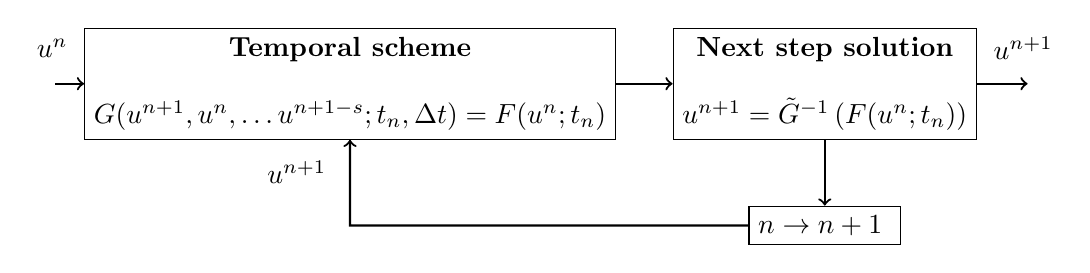
\begin{tikzpicture}[scale=0.9]
		\node[rectangle](0) at (-4.3,0) {};
		\node[rectangle](un) at (-4.2,0.5) {$\vect{u}^{n}$};
		\node[rectangle](f) at (9.7,0) {};
		\node[rectangle](un1) at (9.5,0.5) {$\vect{u}^{n+1}$};
		\node[rectangle](e) at (-0.75,-1.25) {$\vect{u}^{n+1}$};
	%	\node(ab) at (4,0.5) {$\vect{\tilde{G}}^{-1}$};
		
		\tikzstyle{every node}=[draw, align=center, rectangle ]
		\node(a) at (0,0) {\textbf{Temporal scheme} \\ \\$\vect{G}(\vect{u}^{n+1}, \vect{u}^{n}, \ldots \vect{u}^{n+1-s};t_n, \Delta t)=\vect{F}(\vect{u}^n;t_n)$};
		
		
		\node(b) at (6.7,0) {\textbf{Next step solution} \\ \\$\vect{u}^{n+1}=\vect{\tilde{G}}^{-1} \left(\vect{F}(\vect{u}^n;t_n)\right)$};
		
		\node(c) at (6.7,-2) {$n \rightarrow n +1 $ 
		};
		
		\draw [->, thick = 1 pt] (c) -- (0,-2) -- (a) ;
		
		\foreach \from/\to in {0/a,a/b,b/c,b/f}
		\draw [->, thick = 1 pt] (\from) -- (\to) ;%node[midway] {\from--\to};
		
		
		\end{tikzpicture}
		\caption{Resolution algorithm for Cauchy problems.}
		\label{fig:CauchyProblemAlgorithm}
	\end{figure}
}


\newcommand{\RKstepsize}[1]
{
	\functiongraph
	{}{}
	{ xlabel = $h$, ylabel = $f$, xmin = 0, xmax = 0.5, ymin = 0, ymax = 0.5, no marks, samples = 2 , view ={0}{90}, axis lines=left, ticks=none }
	{}
	{}
	{ 
		\curveplot{0:0.5}{0:0.4}{}{x}{x}{0}
		\curveplot{0:0.5}{0:0.4}{red}{x}{0.8*x}{0}
		\curveplot{0:0.5}{0:0.4}{blue}{x}{0.7*x}{0}
		
		\curveplot{0:0.2}{0:0.2}{dashed, green}{0.2}{y}{0}
		\curveplot{0.2:0.25}{0:0.2}{dashed, green}{x}{0.2}{0}
		
		\curveplot{0.2:0.25}{0:0.25}{dashed, green}{0.25}{y}{0}
		\curveplot{0.25:0.36}{0.23:0.25}{dashed, green}{x}{0.25}{0}
		\curveplot{0.36:0.47}{0:0.25}{dashed, green}{0.36}{y}{0}
		%		\curveplot{0.4:0.42}{0:0.4}{dashed}{0.4}{y}{0}
		%		\curveplot{0.6:0.62}{0:0.4}{dashed}{0.6}{y}{0}
		%		\node[] at (0.27, 0.03)   (a) {$h_0$};
		\node[] at (0.40, 0.02)   (a) {$h_0$};
		
		
		\node[] at (0.27, 0.02)   (a) {$h_1$};
		\node[] at (0.18, 0.02)   (a) {${h_2}$};
		\node[blue] at (0.2, 0.28)   (a) {$f_0(h_0)$};
		\node[red] at (0.13, 0.22)   (a) {$f_1(h_1)$};
		
		
		\node[] at (0.085, 0.48)   (a) {$f=h$};
		\node[red] at (0.1, 0.43)   (a) {$f_1=a_1 h$};
		\node[blue] at (0.1, 0.38)   (a) {$f_0=a_0 h$};
		%		\node[] at (0.42, 0.035)   (a) {$\tilde{h}$};
		%		\node[] at (0.63, 0.03)   (a) {$h_0$};
		%		\node[] at (0.57, 0.43)   (a) {$f(h_0)$};
	}
	{#1}
}

\newcommand{\StepSizeRK}[1]
{
	\begin{figure}[H]
		%		\hspace{-0.5cm}
		\begin{tikzpicture}
		\node[rectangle](0) at (-2.5,0) {};
		\node[rectangle](hi) at (-2.,0.5) {$h_i$};
		\node[rectangle](f) at (9,0) {};
		\node[rectangle](yes) at (8.3,0.25) {Yes};
		
		\node[rectangle](h) at (8.4,-0.4) {$h=h_{i}$};
		\node[rectangle](hi1) at (-0.75,-1.25) {$h_{i+1}$};
		\node(ab) at (2.15,0.4) {$\norm{ \vect{T}^{n+1}_i }$};
		\node(no) at (6.4,-1.3) { No };
		\tikzstyle{every node}=[draw, align=center, rectangle ]
		\node(a) at (0,0) {\textbf{Cauchy } \\ \textbf{problem} };
		
		
		\node[diamond, aspect=2](c) at (6,0) { $\norm{ \vect{T}^{n+1}_i } \leq  \epsilon$ ? 
		};
		
		\node(d) at (6,-2) {$h_{i+1} = a_i h_i $ 
		};
		
		\draw [->, thick = 1 pt] (d) -- (0,-2) -- (a) ;
		
		\foreach \from/\to in {0/a,a/c,c/d,c/f}
		\draw [->, thick = 1 pt] (\from) -- (\to) ;%node[midway] {\from--\to};
		
		
		\end{tikzpicture}
		\caption{Step size selection process for embedded Runge-Kutta method.}
		\label{#1}
	\end{figure}
}
 \newcommand{\VanDerPooleERKFlow}[1]
{
	\mixgraphs{$x$}{$\dot{x}$}
	{mark repeat = 301, legend columns = 2 , legend pos =south east, ymax = 4.2, ymin = -4.2}
	{./doc/chapters/Cauchy_problem/figures/VanDerPooleERK.plt }
	{\texttt{RK87},\texttt{Fehlberg87}}
	{
		1/2,%
		3/4%
	}
	{}{#1}
}

 \newcommand{\VanDerPooleERKx}[1]
{
	\mixgraphs{$t$}{$x$}
	{mark repeat = 20, legend columns = 2, legend pos =north east }
	{./doc/chapters/Cauchy_problem/figures/VanDerPooleERK.plt }
	{}
	{
		0/1,%
		0/3%
	}
	{}{#1}
}


 \newcommand{\HenonHeilesGBSxy}[1]
{
	\mixgraphs{$x$}{$y$}
	{no marks, legend columns = 2 }
	{./doc/chapters/Cauchy_problem/figures/HenonHeilesGBS.plt }
	{}
	{
		1/2%
	}
	{}{#1}
}

 \newcommand{\HenonHeilesGBSxVx}[1]
{
	\mixgraphs{$x$}{$p_x$}
	{no marks, legend columns = 2 }
	{./doc/chapters/Cauchy_problem/figures/HenonHeilesGBS.plt }
	{}
	{
		1/3%
	}
	{}{#1}
}

 \newcommand{\HenonHeilesGBSyVy}[1]
{
	\mixgraphs{$y$}{$p_y$}
	{no marks, legend columns = 2 }
	{./doc/chapters/Cauchy_problem/figures/HenonHeilesGBS.plt }
	{}
	{
		2/4%
	}
	{}{#1}
}

 \newcommand{\HenonHeilesGBSVxVy}[1]
{
	\mixgraphs{$p_x$}{$p_y$}
	{no marks, legend columns = 2 }
	{./doc/chapters/Cauchy_problem/figures/HenonHeilesGBS.plt }
	{}
	{
		3/4%
	}
	{}{#1}
}


%%%%%%%% STABILITY REGIONS %%%%%%%%%%%%


 \newcommand{\RKstability}[1]
{
	\onecontour{xlabel=$\Re z$,ylabel=$\Im z$, point meta max = 1, colormap/blackwhite}
	{51}
	{./doc/chapters/Cauchy_problem/figures/RKstability.plt }
	{contour filled={number=20}}
	{}
}


 \newcommand{\CashKarpstability}[1]
{
	\onecontour{xlabel=$\Re z$,ylabel=$\Im z$, point meta max = 1, colormap/blackwhite}
	{51}
	{./doc/chapters/Cauchy_problem/figures/CashKarpstability.plt }
	{contour filled={number=20}}
	{}
}



 \newcommand{\nomenclature}
{
 \begin{center}
     \begin{figure}[H]
     	\setlength{\unitlength}{0.08cm}
         \centering
         \vbox{
             \begin{picture}(150,55)
             
             %   \put(0,0){\framebox(150,55)}            
             
             
             \drawline [100](10,10)(25,10)              
             \put(10,10){\circle*{1.5}}
             \put(25,10){\circle*{1.5}}
             
             \drawline [100](55,10)(80,10)              
             \put(55,10){\circle*{1.5}}
             \put(80,10){\circle*{1.5}}          
             
             \drawline [100](80,10)(120,10)        
             \put(120,10){\circle*{1.5}}         
             
             
             
             \put(8,5){$t_0$}
             \put(23,5){$t_1$}           
             \put(53,5){$t_{n - 1}$}
             \put(78,5){$t_{n}$}         
             \put(118,5){$t_{n + 1}$}
             
             \put(115,45){$\Delta t_{n} \ = \ t_{n + 1} \ - \ t_{n}$}            
             
             \drawline [20](55,10)(55,17)
             \drawline [20](80,10)(80,17)
             \drawline [20](120,10)(120,17)          
             
             
             
             \put(14.5,15){$\Delta t_0$}
             \put(62.5,15){$\Delta t_{n - 1}$}
             \put(96,15){$\Delta t_{n}$}                     
             
             
             \drawline [20](10,10)(10,17)
             \drawline [20](25,10)(25,17)
             
             \put(13,16){\vector(-1,0){3}}
             \put(22,16){\vector(1,0){3}}
             
             \drawline [20](10,10)(10,17)
             \drawline [20](25,10)(25,17)
             
             \put(61,16){\vector(-1,0){6}}
             \put(74,16){\vector(1,0){6}}            
             
             \put(95,16){\vector(-1,0){15}}
             \put(105,16){\vector(1,0){15}}                  
             
             
             \dashline {2}(10,10)(10,30) 
             \dashline {2}(25,10)(25,40) 
             \dashline {2}(55,10)(55,35) 
             \dashline {2}(80,10)(80,45) 
             \dashline {2}(120,10)(120,25) 
             
             \dashline {2}(25,10)(55,10) 
             
             \put(10,30){\circle*{1.5}}
             \put(25,40){\circle*{1.5}}          
             \put(55,35){\circle*{1.5}}
             \put(80,45){\circle*{1.5}}      
             \put(120,25){\circle*{1.5}} 
             
             \put(8,33){$U^{0}$}         
             \put(23,43){$U^{1}$}                                                                          
             \put(53,38){$U^{n - 1}$}    
             \put(78,48){$U^{n}$}    
             \put(118,28){$U^{n + 1}$}                           
             
             
             \end{picture} 
             \caption{Partition of the temporal domain}
             \label{nomenclature}
         }
     \end{figure}
 \end{center}
} 